% !TEX root = thesis.tex

\chapter{A Large Scale Corpus with Wide Spectrum of Social Signal Measurements}
\label{chapter:dataset}
Availability of a large-scale dataset is essential to computationally analyze the nonverbal communication in a data-driven manner. Despite existing datasets that provide measurements for human motion and behaviors~\cite{carletta2005ami, Lepri-12, Zen-10,Cristani-11, SALSA-15, h36m_pami}, there is no dataset that satisfies the following core requirements for understanding non-verbal human behaviors: (1) capturing 3D full body motion at high-resolution (including face, body, and hands); (2) capturing signals of naturally interacting groups (more than two people to include attention switching); and (3) collecting the data at scale. The limited availability of the dataset motivates us to build a new dataset that contains social interactions among hundreds of interacting groups with the full-spectrum of 3D body motion measurements. The key properties of our dataset are as follows:
\begin{itemize}
	\item Our dataset contains naturally interacting multiple people in a negotiation game scenario that is carefully designed in the collaboration with pychologists
	\item No behavioral restriction is instructed to participants during the capture, and subjects are randomly recruited
	\item Our dataset contains videos from over 500 views. All cameras are calibrated and temporally synchronized
	\item High-resolution social signals are measured using markerless motion capture~\cite{joo2017panoptic, joo2018}, including 3D anatomical landmarks for body, face, hands, and 3D point clouds
	\item Our dataset contains audio recording the voice signal for each subject, which is synchronized with videos, as well as annotated speaking status for each individual
\end{itemize}

The objective of our dataset is to study the correlation among subtle socials signals transmitted during a social situation. To make human behaviors more coherent, we define a social scenario so that all the subjects are in the same social situation. Capturing the natural motion of the subjects is crucial in our study, so we use the state-of-the art markerless motion capture methods in the CMU Panoptic Studio~\cite{joo2017panoptic, joo2018}. Importantly, the multi-modal property of our dataset enables us to study the correlation among various input and output signals. Our dataset is captured under a university-approved IRB protocol and will be publicly available for research purposes.
%\begin{figure}
%	\centering
%	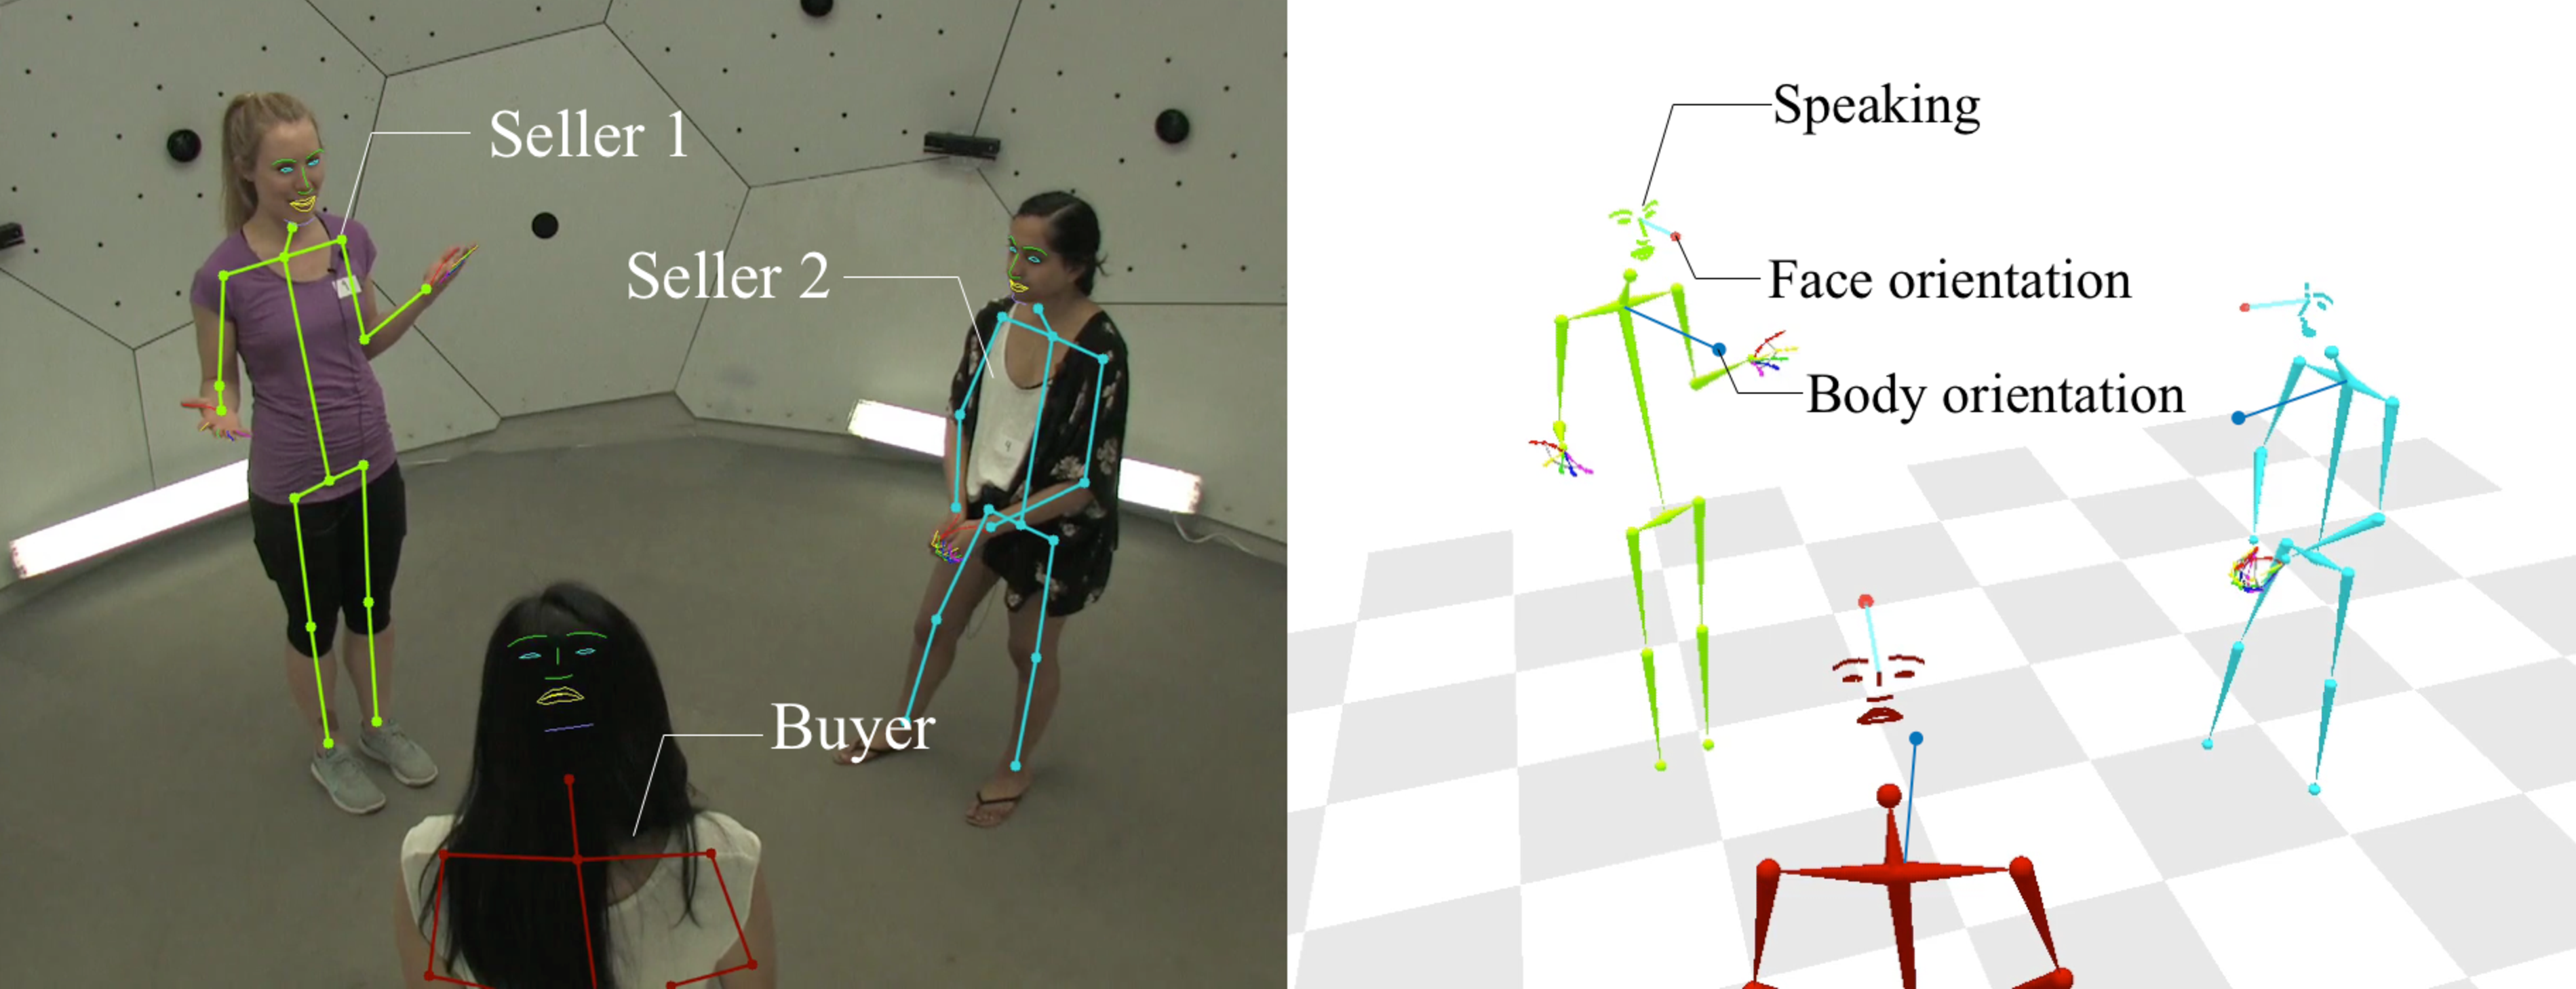
\includegraphics[width=\linewidth]{ssp_fig/haggling_ex}
%	\caption{An example of the haggling sequence. (Left) an example scene showing two sellers and one buyer. (Right) Reconstructed 3D social signals showing body, face, and 3D hand motion.} 
%	\label{fig:haggling_example}
%\end{figure}

\begin{figure}
	\centering
	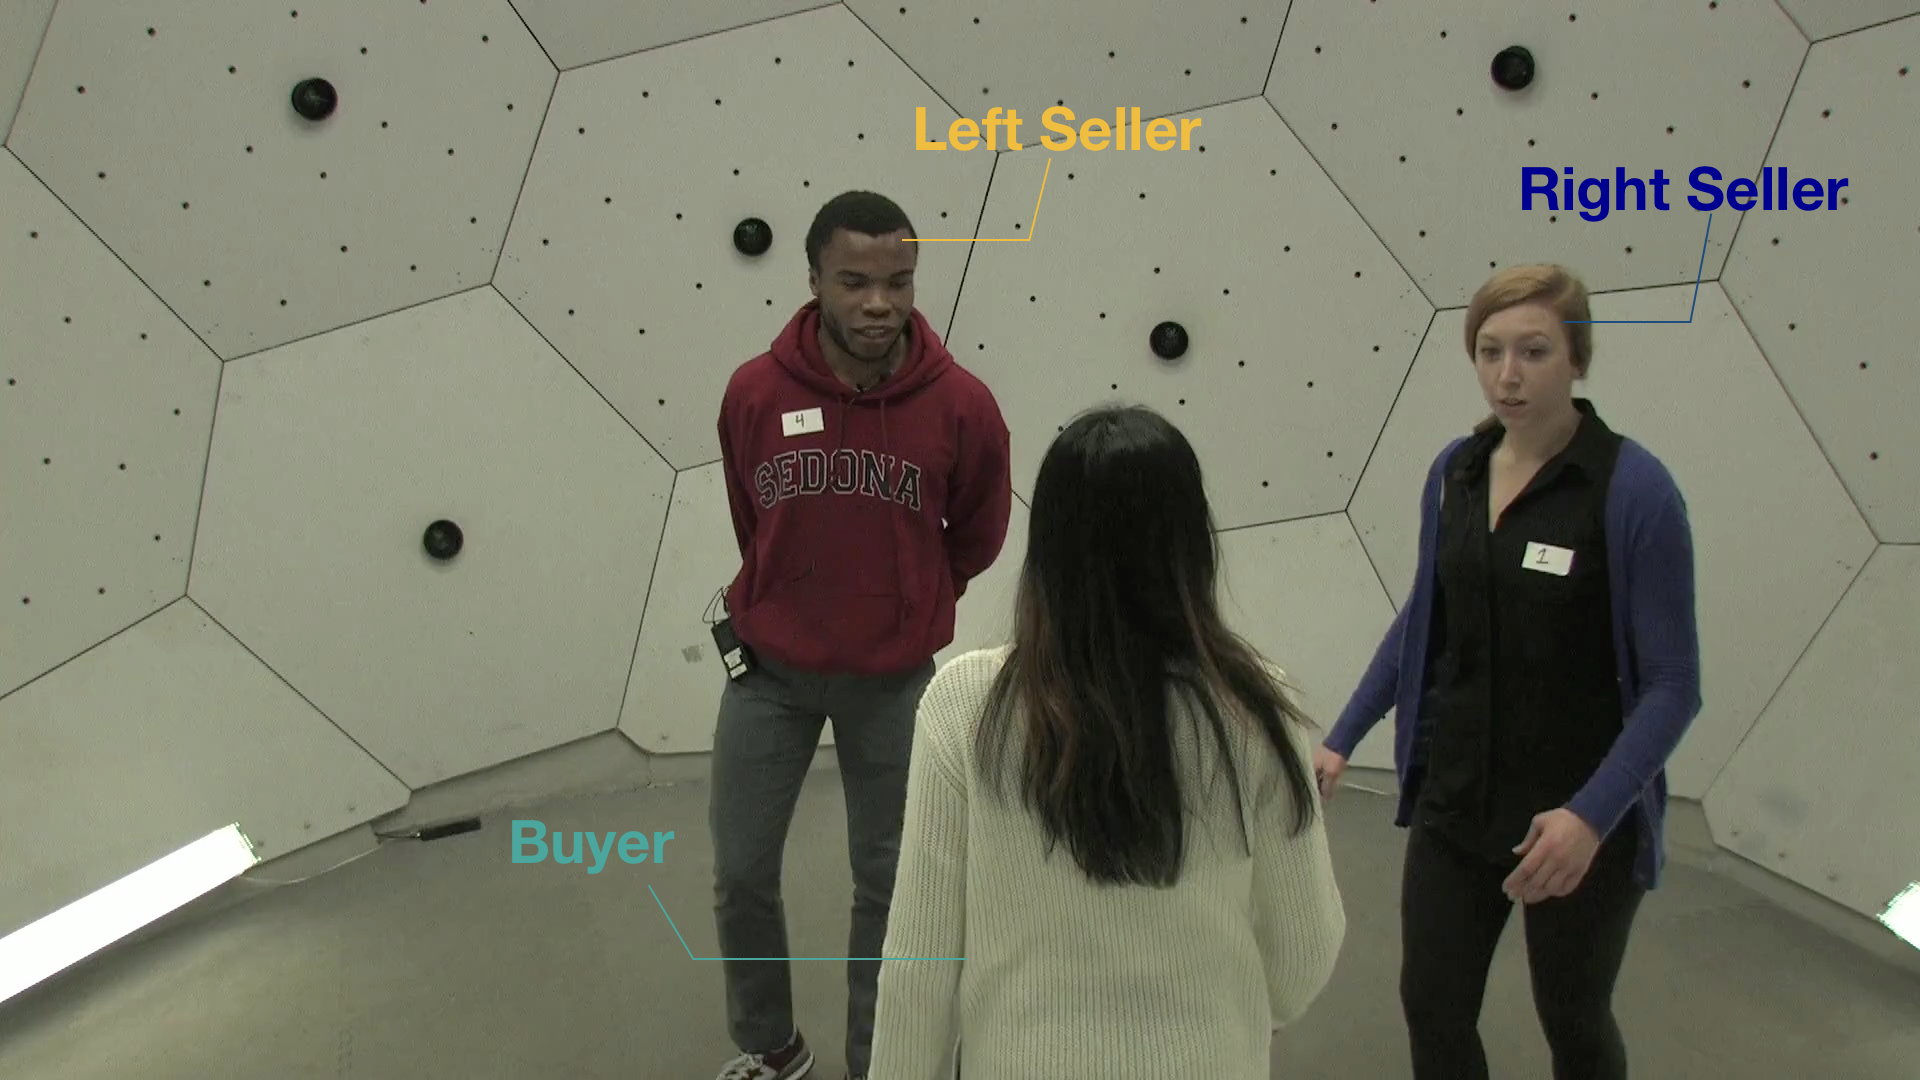
\includegraphics[trim=300 0 0 0,clip,width=0.49\linewidth]{ssp_fig/haggling_ex_input}
	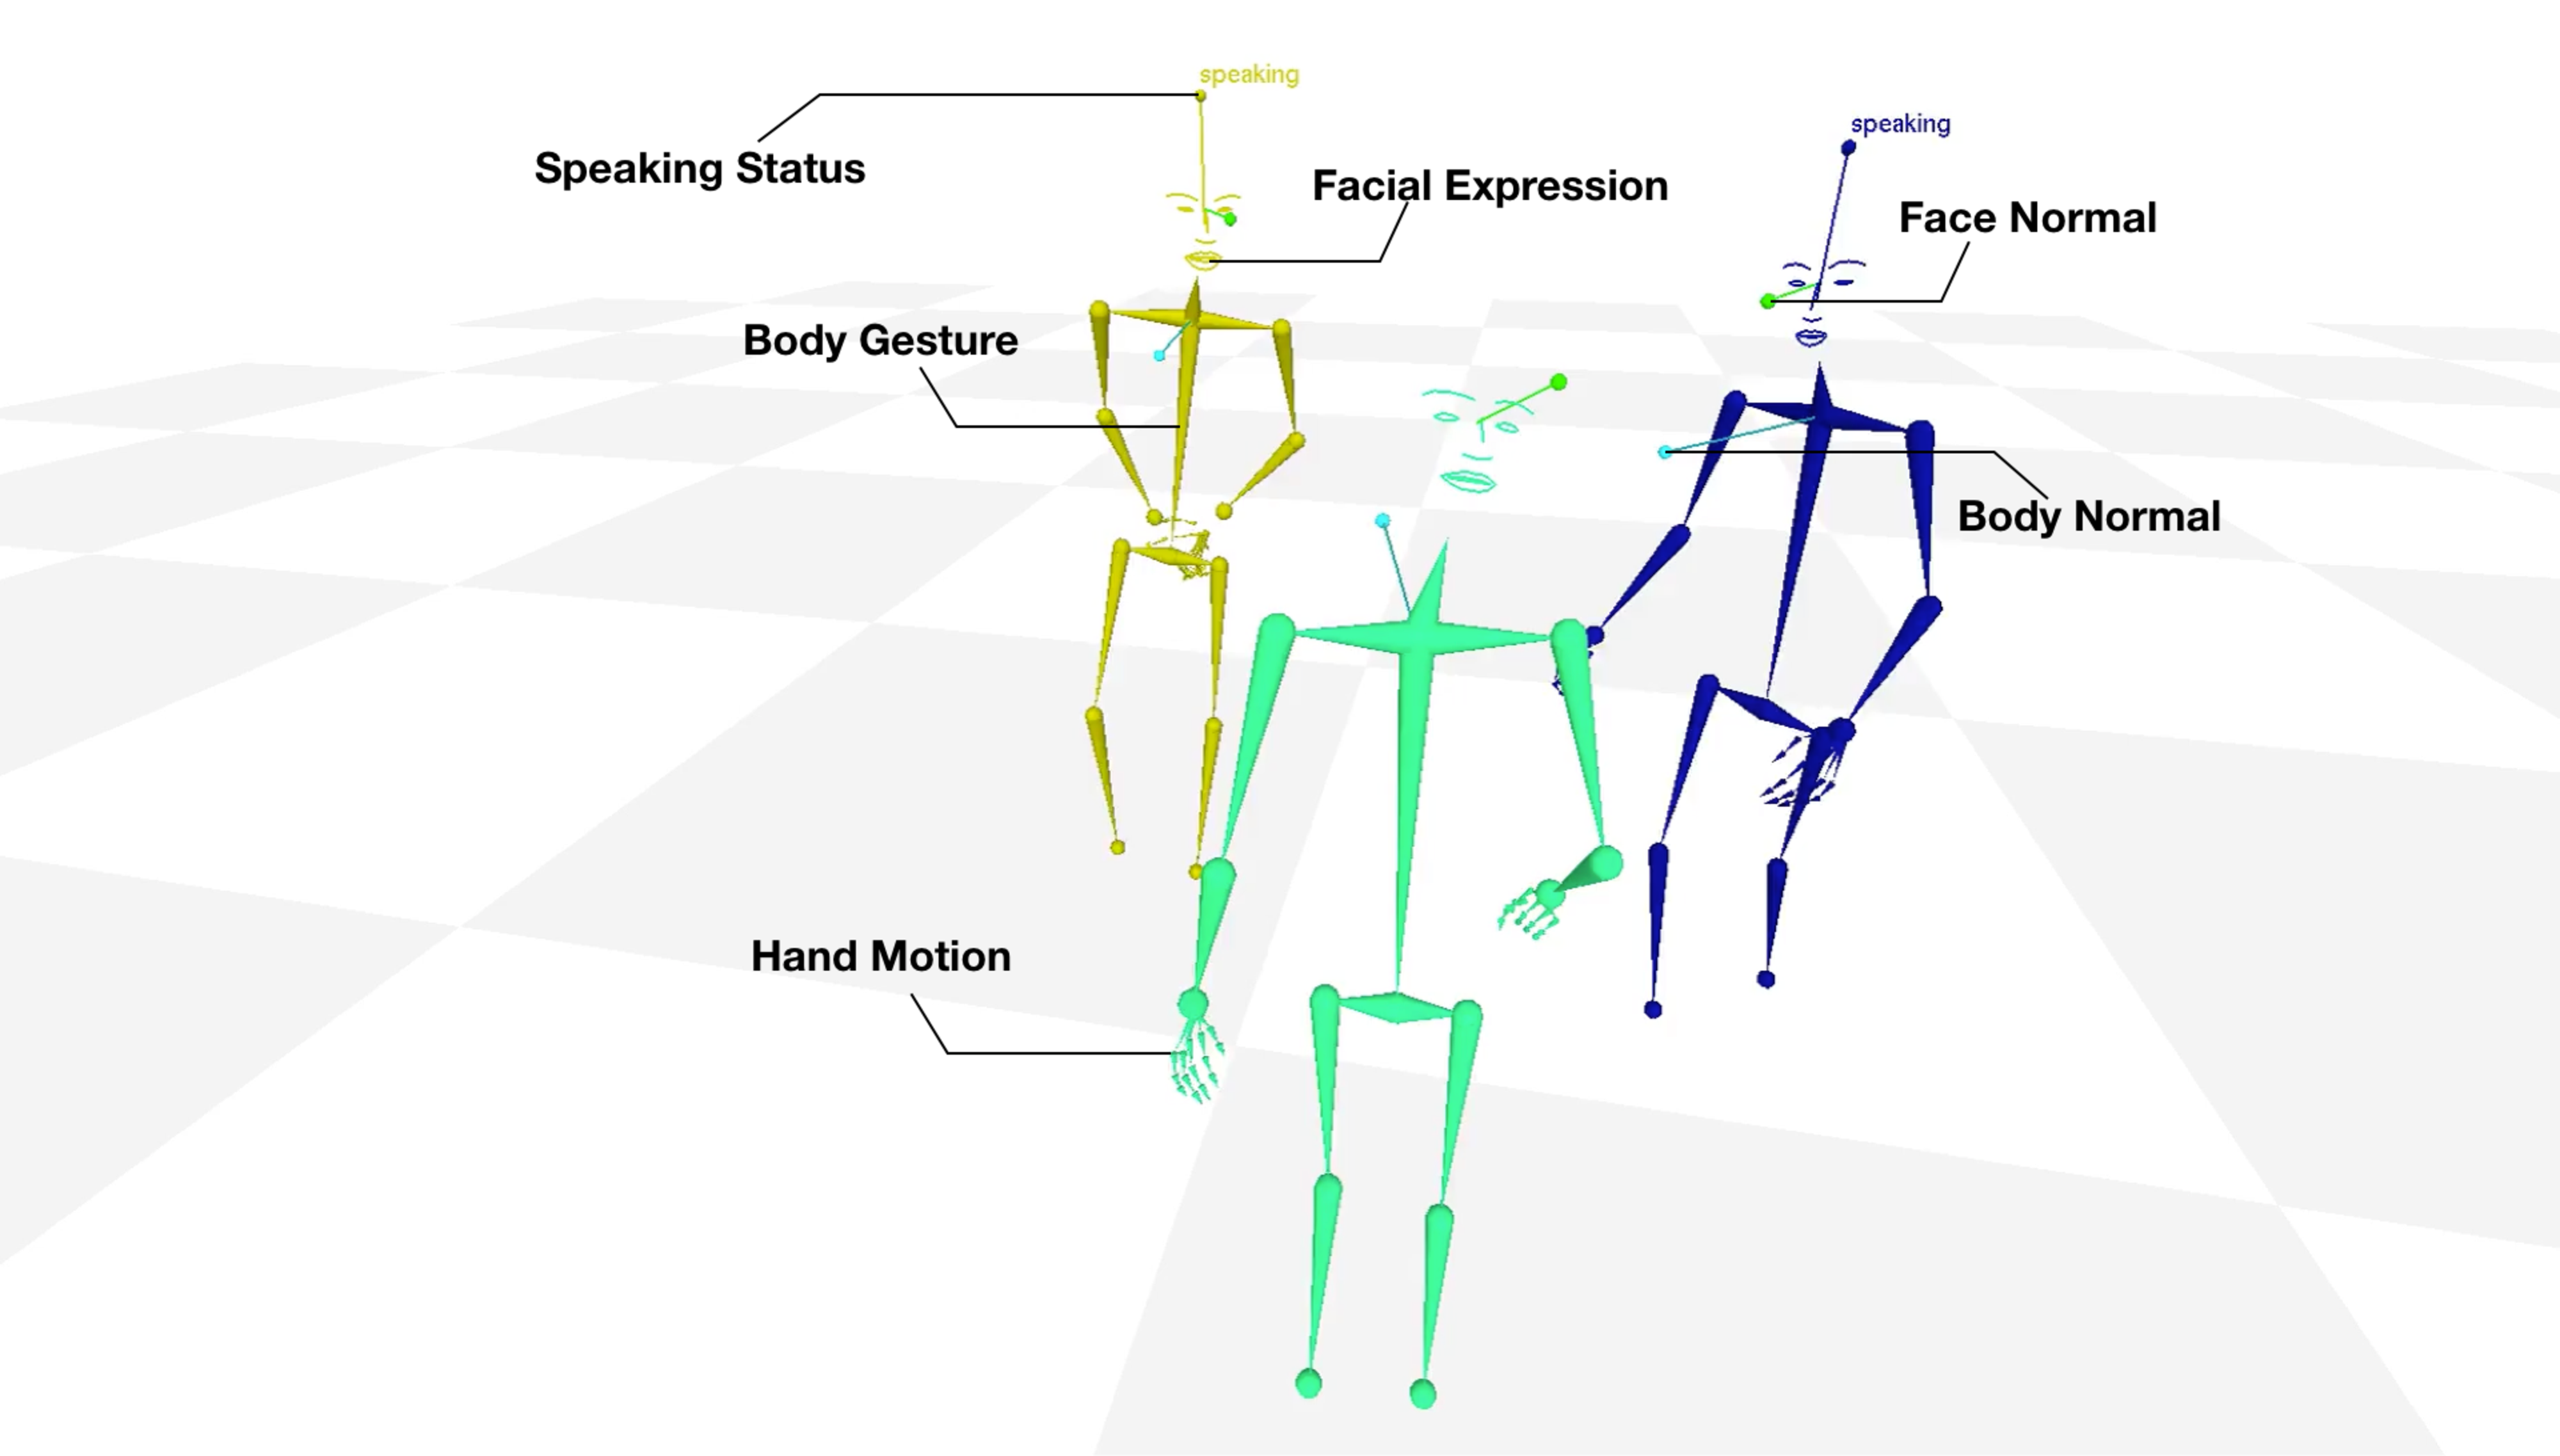
\includegraphics[trim=300 0 0 0,clip,width=0.49\linewidth]{ssp_fig/haggling_ex_measure}
	\caption{An example of the haggling sequence. (Left) an example scene showing two sellers and one buyer. (Right) Reconstructed 3D social signals showing body, face, and 3D hand motion.} 
	\label{fig:haggling_example}
\end{figure}

\section{Related Work}

%\subsection{Social Signal Processing DB:}


\begin{figure}
	\centering
	\frame{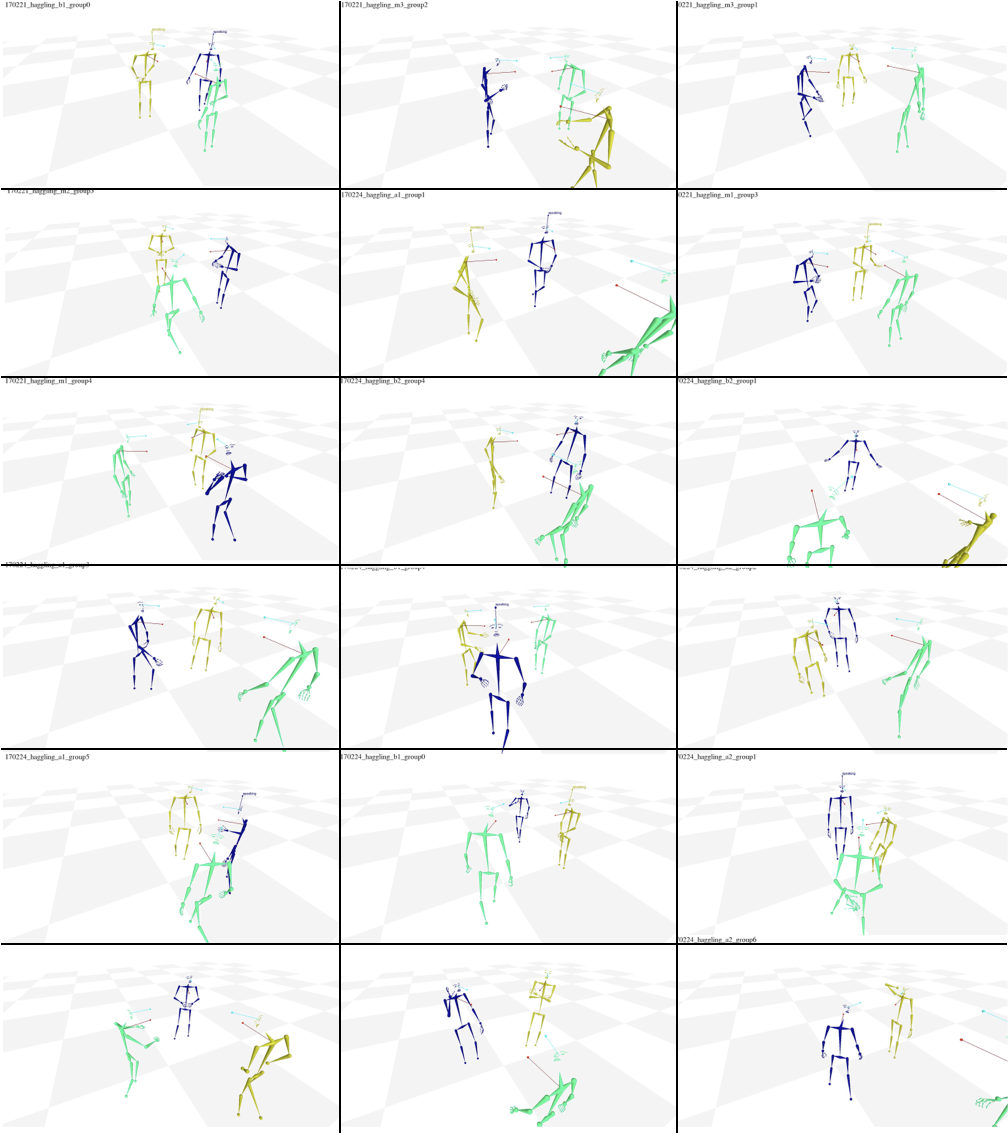
\includegraphics[width=\textwidth]{ssp_fig/haggling_examples}}
	\caption{Example scenes of haggling sequences.} 
	\label{fig:haggling_others}
\end{figure}


%Emilya: Emotional body database
%FABO corpos
%GEMEP corpus: actor behave
%Modeling human affective postures: an information theoretic characterization of posture features
%\subsection{Affective Posture Database:}
A research domain considers to recognize emotions in body gestures. Almost all databases in this domain are collected from actors where actors are instructed to behave certain emotions~\cite{gunes2006bimodal, banziger2012introducing, de2004modeling}. 

%\subsection{Face-to-face Social Interacton Database:}
%SALSA: alameda2016salsa
%AMI meeting db: mccowan2005ami

%Free-standing
%Space speaks: towards socially and personality aware visual surveillance

%Other device:
%13. Pentland, A.: Looking at people: Sensing for ubiquitous and wearable computing.
%IEEE PAMI. 22(1) (2000) 107–119
%14. Choudhury, T., Pentland, A.: The sociometer: A wearable device for understanding
%human networks. In: CSCW - Workshop on ACCUCE. (2002

%\textbf{Social Signal Dataset:}
How to measure and collect nonverbal signal data is important to pursue a data-driven approach for our goal.  A research domain considers to recognize emotions in body gestures. Almost all databases in this domain are collected from actors where actors are instructed to behave certain emotions without actual social interaction~\cite{gunes2006bimodal, banziger2012introducing, de2004modeling}. Few datasets contain socially interacting group motion~\cite{mccowan2005ami, zancanaro2006automatic, lepri2012connecting, rehg2013decoding}. The scenes in these datasets are often in a table setup, limiting free body movement and capturing the upper-body only. There are datasets that capture free-standing conversational groups (e.g., cocktail party)~\cite{Zen-10, Cristani-11, alameda2016salsa, farenzena2009social}, but these only contain location and orientation measurements for the people, introduced to study the social formation or coarse category level recognition tasks (e.g., speaker, personality, or role recognition).

% Datasets providing rich 3D body motion information captured with motion capture techniques exist, but they contains single subjects' motion only\cite{gross2001cmu, h36m_pami, sigal2010humaneva}. More recently, however, full body motion data of interacting groups using a large number of camera system was proposed for social interaction capture~\cite{Joo-15}. This work shows a potential in collecting a large scale social interaction data without the usual issues caused by wearing a motion capture suit and markers.

%\subsection{Human Motion Capture Database:}
Datasets providing rich 3D body motion information captured with motion capture techniques exist, but they contains single subjects' non-social motion only\cite{gross2001cmu, h36m_pami, sigal2010humaneva}. 

Notably, there is not previous work where socially interacting groups are non-intrusively captured with full body motion capture measurements. 


\begin{table}[h]
	\centering
	
	\begin{tabular}{ c| c | c  }
		\hline	
		Items & Seller 1  &  Seller 2\\
		\hline	
		\hline	
		Phone &  \makecell{Light weight \\ Medium storage}    & \makecell{Medium weight\\ Large storage}\\
		\hline			
		Laptop &  \makecell{Light weight \\ Medium speed}    & \makecell{Medium weight\\ Fast speed}\\
		\hline			
		Tablet PC &  \makecell{Large storage\\ Medium speed}    & \makecell{Medium storage\\ Fast speed}\\
		\hline	
		Speaker &  \makecell{High quality audio\\ Wired}    & \makecell{Medium quality audio\\ Wireless}\\
		\hline	
	\end{tabular}
	\caption{Example of items assigned to sellers}
	\label{table:haggling_items}
\end{table}


\section{The Haggling Game Protocol}
To evoke natural interactions, we involved participants in a social game named the \emph{Haggling} game. This game induces a variety of rich non-verbal signals in participants. In our captures, subjects were informed of the rules of the game but were otherwise not instructed about how to behave, nor was their clothing or appearance controlled. They were also not initially aware of our research goals to avoid potential biases in their gestures. The majority of the sequences are captured with people randomly recruited from a university campus. We invent this haggling game to simulate a haggling situation among two sellers and a buyer. The triadic interaction is chosen to include interesting social behaviors such as turn taking, and attention changes, which are missing in dyadic interactions~\cite{rehg2013decoding}. During the game, two sellers are promoting their own comparable products for selling, and a buyer makes the decision about which product he/she buys between the two. They are given a minute for the haggling, and the seller who has sold his/her product is awarded $\$5$. To maximize the influence of each seller's behavior on the buyer's decision-making, the items assigned to sellers are the same type of product with slightly different properties. We provide simple written descriptions to sellers about the items 1 minute before the game. Over the 8 days of captures, 122 subjects participated and 180 haggling sequences were captured (about 3 hours data). The captured sequences contain a lot of voluntary social behaviors of diverse people in a common social context (an example scene is shown in Fig.~\ref{fig:haggling_example}. Note that the capture space does not contain other objects which may distract the motion of the target, so we can assume no $X_e(t)$ is necessary in our social signal prediction problem.







\section{Social Signal Measurements}
We use the Panoptic Studio System to reconstruct 3D anatomical keypoints of multiple interacting people~\cite{joo2017panoptic, joo2018}. As a key advantage, the method does not require attaching sensors or markers on subject's body, and no behavior restrictions nor initialization poses are needed from the subjects. As output, the system produces 3D body motion $\mathbf{J(t)}$, 3D face motion $\mathbf{F(t)}$, and 3D hand motion $\mathbf{H(t)}$ for each individual at each time $t$. From this measurement, we additionally compute the body orientation $\theta(t)$ and face orientation $\phi(t)$ by finding the 3D normal direction of torso and face. These orientations are computed only on the $x$-$y$ plane with respect to the $y$-axis. We decouple the global location $x$ and body orientation $\theta$ from the body motion capture results, following previous work~\cite{jain2016structural, holden2016deep}, and $\mathbf{J(t)}$ only contains body motions in the person-centric coordinate (root joint is at the origin and body is facing the $z$ direction). An example scene is shown in Fig.~\ref{fig:haggling_example}. The voice data $V(t)$ of each individual is also recorded by wireless microphones assigned to each individual. From the audio signal, we manually annotate a binary speaking label $\mathbf{S}(t) \in \{0,1\}$ describing whether the target subject is speaking (labelled as $1$) or not speaking (labelled as $0$) at time $t$.
% In summary we measure the following signals for each individual:
%\begin{equation}
%[ \mathbf{x}, \boldsymbol{\theta}, \boldsymbol{\phi}, \mathbf{J}, \mathbf{F}, \mathbf{H}, \mathbf{V}, \mathbf{S} ].
%\label{equation:measurement}
%\end{equation}


\begin{figure}
	\centering
	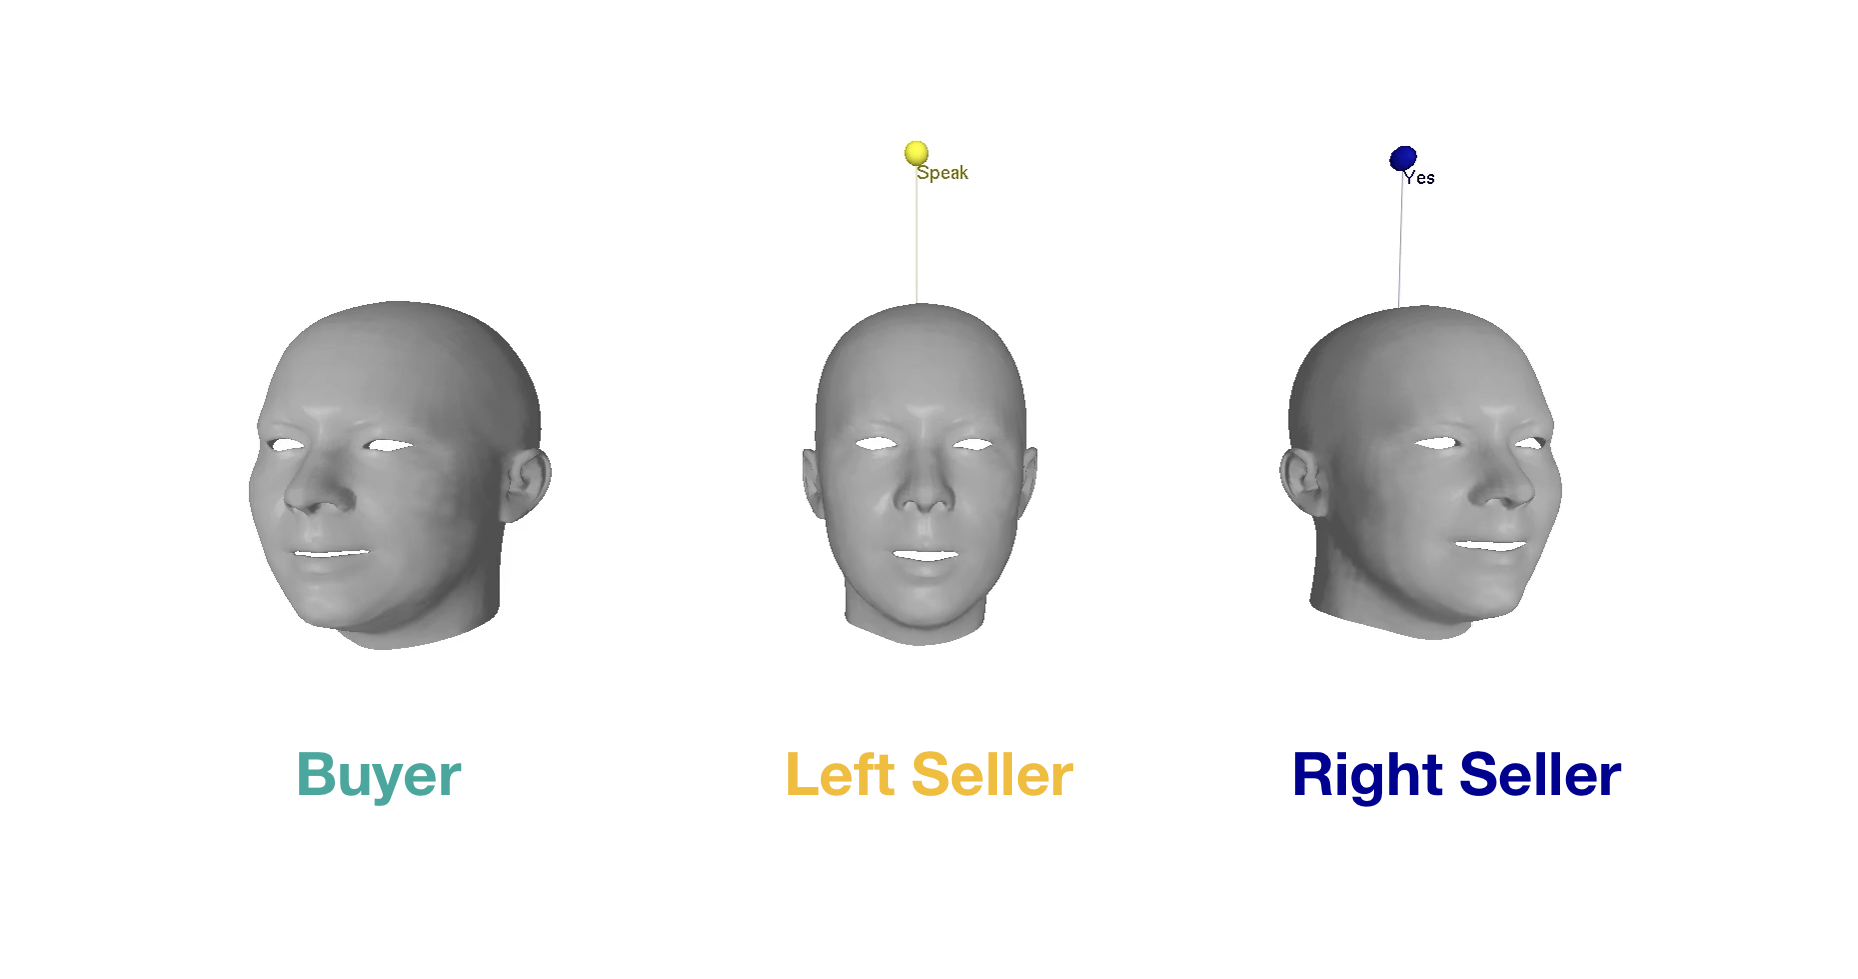
\includegraphics[width=0.49\textwidth]{ssp_fig/haggling_ex_face}
	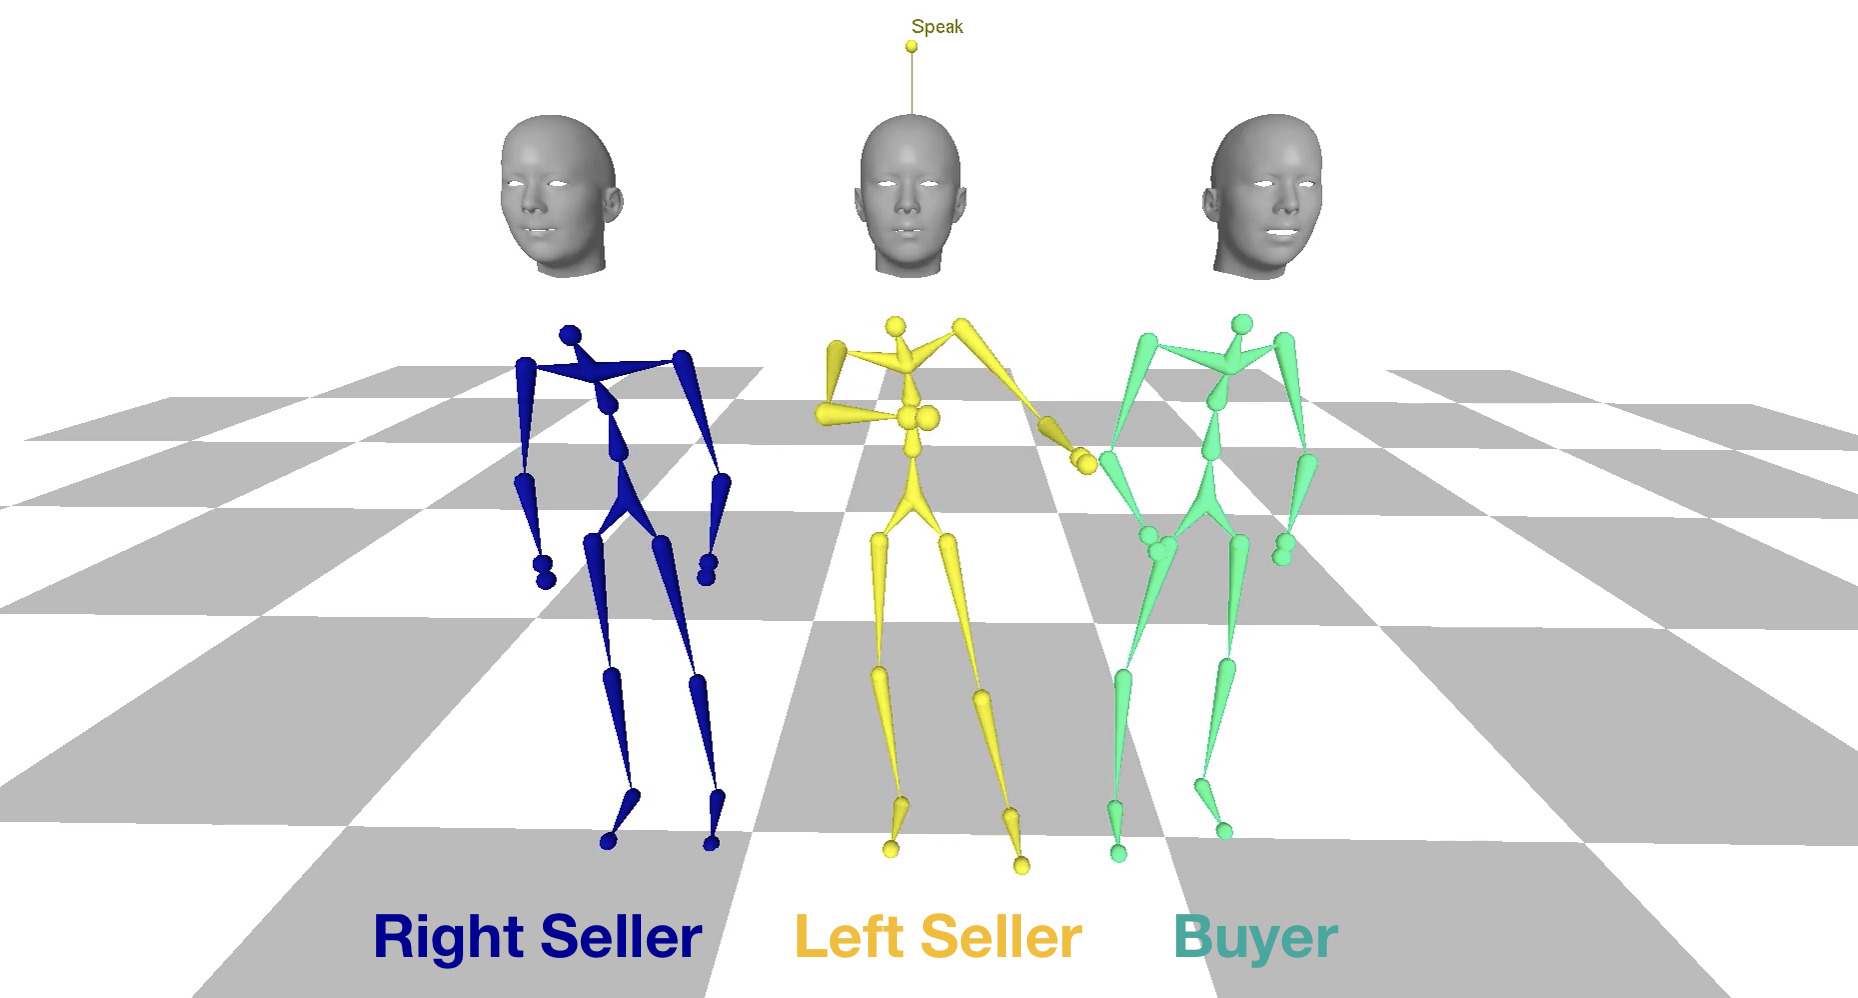
\includegraphics[width=0.49\textwidth]{ssp_fig/haggling_ex_facebody}
	\caption{Visualizing part of social signals. (Left) Visualizing face and speaking annotation, (Right) Visualizing face, body, and speaking annotation excluding social formation.} 
	\label{fig:haggling_measurement_vis}
\end{figure}



\section{Other Social Game Sequences}

%\section{Social Game Protocols}
%To evoke natural interactions, we involved participants in various games: \emph{Ultimatum}, \emph{Mafia}, \emph{Haggling}. The first two games are used in experimental economics and psychology to study conflict and cooperation, and the Haggling game also induces a variety of rich non-verbal signals in participants. In our captures, subjects were informed of the rules of the game but were otherwise not instructed about how to behave, nor was their clothing or appearance controlled. They were also not initially aware of our research goals to avoid potential biases in their gestures. The majority of the sequences are captured with people randomly recruited from a university campus. The detailed game procedures are described in this section.

\paragraph{Ultimatum.} Ultimatum is a bargaining game that was first experimentally studied by G\"uth et al.~\cite{Guth-82} and has subsequently become among the most studied games in experimental economics~\cite{Chaudhuri-09}. The game consists of two bargainers who are given a certain amount of money to split ($\$10$ in our experiment). One bargainer, referred to as the proposer, suggests a split of the money, and the other bargainer, referred to as the responder, either accepts the split (and both receive money accordingly) or rejects the split (and neither receive anything). Unlike researchers in experimental economics and game theory, we are interested in evoking interactions rather than predicting outcomes of the game, and we therefore make several adjustments to the usual set up of the game. First, we organized participants into teams of proposers and responders (e.g., two proposers and two responders, or four proposers and one responder). Second, we introduced a one minute, face-to-face discussion phase where the participants discuss what they should do (including both inter- and intra-team discussion). One the discussion phase is over, the proposers suggested a split, which the responders either accept or reject without discussion. Third, we did not control for prior acquaintance. Before each experiment, the subjects were introduced to the game informally, with oral instructions explaining the rules. The proposer(s) entered the eventspace first, followed by the responder(s). 

%
%\subsection{Prisoner's Dilemma} Prisoner's dilemma is a game that is originally framed by Merrill Flood and Melvin Dresher, and formalized by Albert Tucker. Two groups are arrested and they are given a Faustian bargain. Each group may betray the other group. If both group remain silent, both will get less penalty, but if only one group betray the other, the other group will be punished harsh while the betrayers got punished least. Because betraying the other gives them the least penalty, natural conclusion from the matrix enforce them to betray each other even if cooperation is the best scenario for both of them. In our capture, we organized participants into two teams with three people for each, with a moderator who shows the reward matrix and announces a final decision from players. Players are given two minutes for intra-group and inter-group discussions, and make a conclusion by passing a selected card to the moderator between two options. The decisions from both teams are displayed by the moderator at the same time, and participants were compensated according to the decision in the reward matrix.  

\paragraph{Mafia.} Mafia is a game created by Dimitry Davidoff~\cite{Haffner-99} that involves both conflict and cooperation, and produces dynamically changing alliances and rivalries within a group of people. Within the group, two individuals (usually) are secretly assigned the roles of ``Mafia" and the rest are assigned roles or ordinary Villagers. The goal of the Villagers is to determine who among them is Mafia via discussion. It is a turn-based game that involves the Villagers choosing to ``execute" one player every turn---their best consensus guess at who the mafia players are---following by the Mafia secretly choosing to secretly ``execute" a Villager of their choice. The game is notable in that it requires some players to engage in outright deception, and requires other players to try to infer this via the interaction alone. In our capture, we involved eight players in the studio. One of them is determined as an operator, and two Mafias and five Villagers are secretly assigned via selecting a lottery.  During the game, we gave them approximately a minute to discuss before iterating on each turn. A large number of interesting phenomena were observed, including subtle motion and gestures to suspect or deceive the other group. Participants were compensated $\$10$ for their participation.

%\subsection{Haggling.} We invent this game to simulate a haggling situation among two sellers and a buyer. Two sellers are promoting their own comparable products for selling, and a buyer makes the decision which product he/she buys between the two. They are given a minute for the haggling, and the seller who has sold his/her product are awarded $\$5$. To avoid any bias caused by personal preference of buyers about the items, the items provided to sellers are simple descriptions of a same type of product but comparably different properties\footnote{We adjusted the game rule multiple times. In old sequences, sellers are given actual objects for selling}. Our recent captures mainly focus on this game due to its simple social settings, and short durations. To this end, we have invited 122 participants and 180 haggling sequences are captured. 
%
%\subsection{007 Bang.} 007-bang game is a party game originated from Korea. Players are located in a circular form, and a turn is started from a starting person who points at someone in the group by hand saying "0". The pointed person, then, points at someone with saying "0" again, and the next pointed person does the same thing with saying "7" at this time, making "007" in turn. The pointed person by the "7" now points someone with saying "bang", and the left and the right person of the finally shot person by the "bang" raise their hands and shout "ah". This game tries to make people confused, because the finally shot person unconsciously tends to raise his/her hands, or the people next to the finally shot person easily forget their required actions. The people who make mistake get a punishment by getting a back massage from others. The next turn is started from the finally shot person. 

\section{Panoptic Studio Database}
Our dataset contains more than 10 hours of sequences, capturing more than 150 participants in total. Categories and detailed information of our dataset is shown in the Table~\ref{table:dataset}.

\begin{table}[h]
	\centering
	\caption{Statistic of Panoptic Studio Dataset}
	\label{table:dataset}
	\begin{tabular}{c| c | c | c }
		\hline	
		Categories & Number of Sequences  & Total Duration~\footnote{This time includes interval between sequences, and thus longer than actual game play time}  & Num. of people per scene \\
		\hline	
		Haggling & 22  & 232m 10s  & 3   \\
		\hline	
		Range of Motion &  - & - & 1   \\
		\hline	
		Ultimatum &  6 & 57m 20s & 2-7   \\
		\hline	
		Mafia &  7 &  83m & 3-8   \\
		\hline	
		Dance&  14& 55m 5s & 1-2   \\
		\hline	
		Musical Instruments& 20 & 73m  & 1-3  \\
		\hline	
		Pose& 33 & 120m  & 1  \\ 
		\hline	
		Toddler& 12 & 26m & 1-3  \\ 
		\hline	
		Hands&  7 &  34m & 1-3  \\ 
		\hline	
		Others& 16 & 20m & 3-15 \\
		\hline	
		\hline	
		Total& 167 & 11h 40m 35s & 1-15\\
		\hline	
	\end{tabular}
\end{table}

\begin{figure}
	\centering
	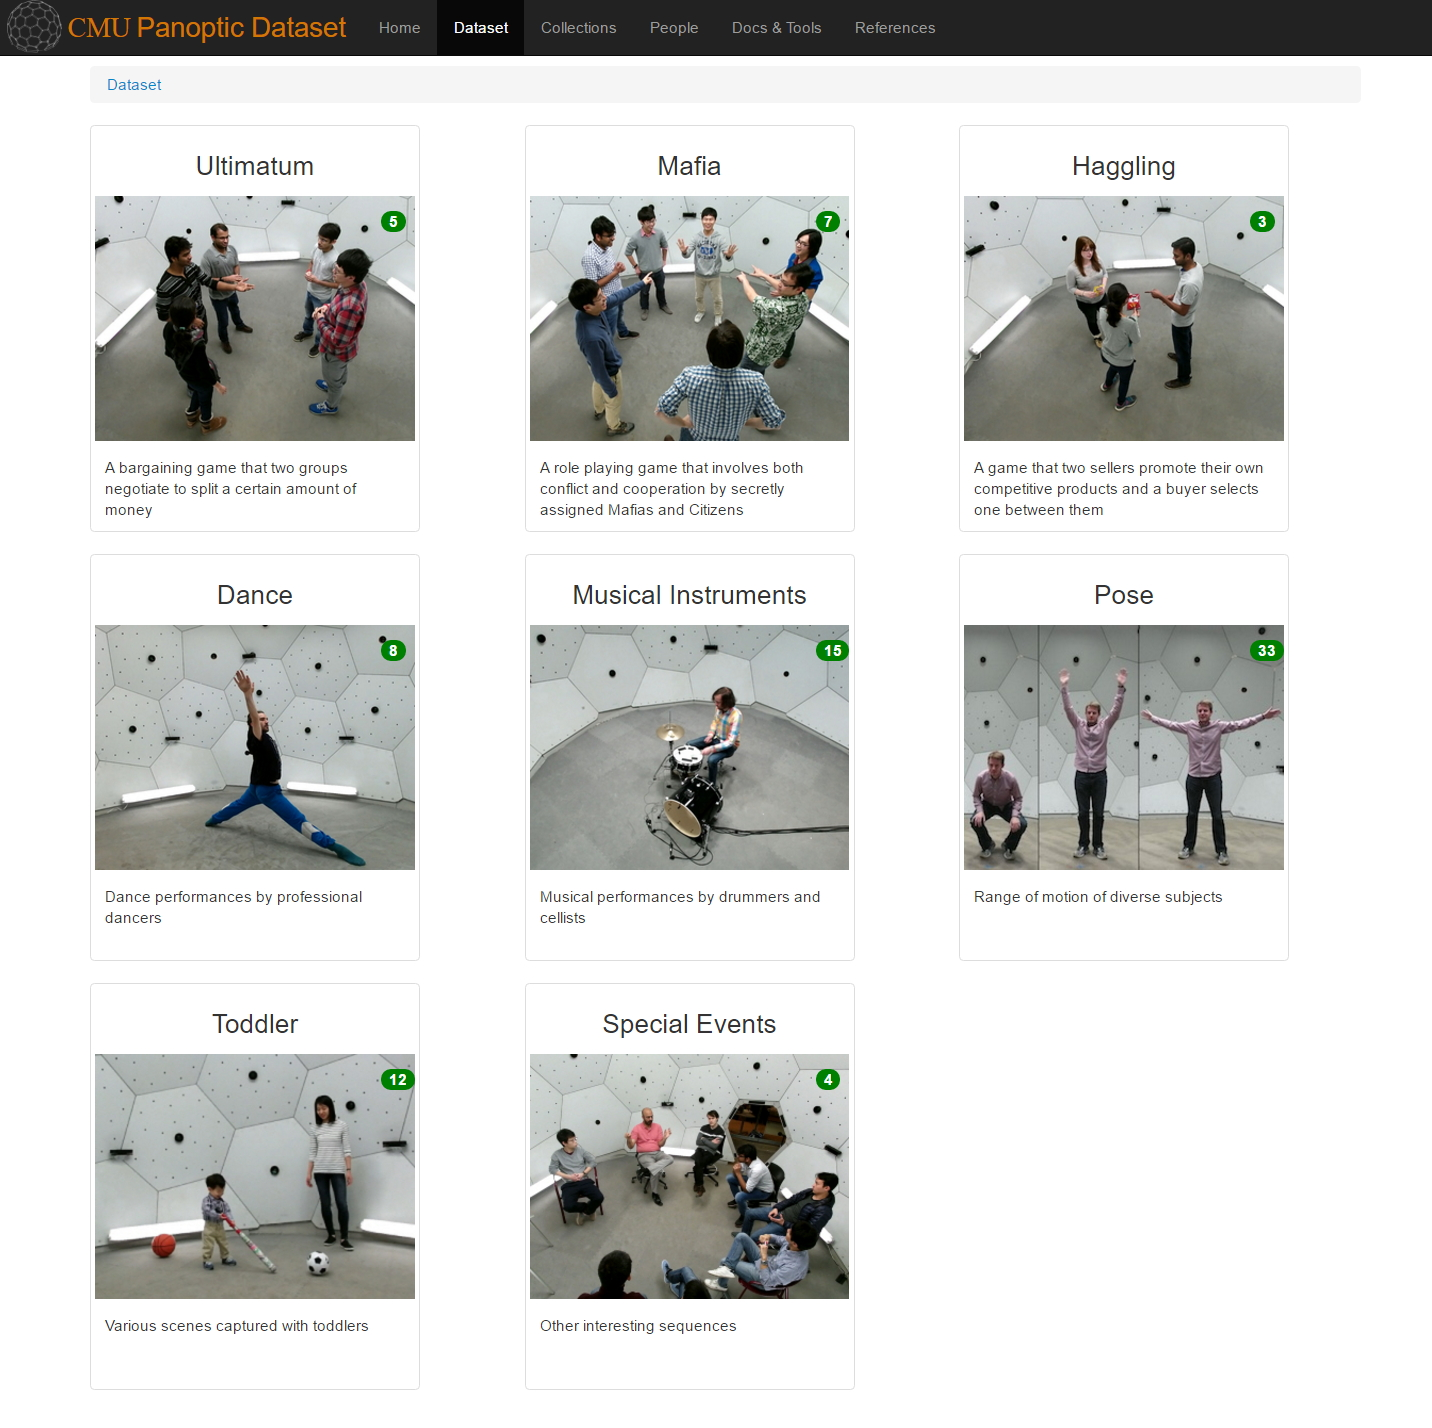
\includegraphics[height=0.95\textwidth]{figures/domedb}
	\caption{The Panoptic Studio Dataset website. We have collected a large number of sequences in various situations. All the 521 sensor measurements as well as reconstructed 3D motion capture results are available.} 
	\label{fig:domedb}
\end{figure}

%\section{Expected Contributions in Computer Vision Community}
%While our dataset is mainly intended to study kinesic signals in social situations, there exist a huge potential in using our dataset for various other computer vision topics. Our dataset contains various type of measurement and automatically generated annotations about dynamically moving human motions. Because all the sensor are temporally and spatially calibration, the dataset can be used as a dataset for various type of computer vision problems to learn the relation among video based scene understanding. 
%
%Over last decade, we have seen that a large number of dataset enables to promote high performance in computer vision algorithms. Yet, still it become a major bottleneck in pursueing new direction of research. For example, annotations for the in-the-wild images collected in the internet is largely limited to relatively simple annotations such as scene category, or bounding boxes. Annotations for richer information such as depth, 3D, videos are not only costly, but also unreliable. In such problem, the available dataset is limited to 3D CAD model, synthetic data, and so on. Due to the reason, the most popular items in computer vision community is stationary object such as bed, chairs, tables, and so on. No rich annotation regarding humans are available, although most of the imagery data is about humans. 
%
%Our dataset provide a potential in that direction. 

\pagebreak